% Template for PLoS
% Version 1.0 January 2009

\documentclass[10pt]{article}

% amsmath package, useful for mathematical formulas
\usepackage{amsmath}
% amssymb package, useful for mathematical symbols
\usepackage{amssymb}

% graphicx package, useful for including eps and pdf graphics
% include graphics with the command \includegraphics
\usepackage{graphicx}

% cite package, to clean up citations in the main text. Do not remove.
\usepackage{cite}

\usepackage{color} 
\usepackage[CaptionAfterwards]{fltpage}
\usepackage{floatrow}
% Use doublespacing - comment out for single spacing
%\usepackage{setspace} 
%\doublespacing

\usepackage{soul}

% Text layout
\topmargin 0.0cm
\oddsidemargin 0.5cm
\evensidemargin 0.5cm
\textwidth 16cm 
\textheight 21cm

% Bold the 'Figure #' in the caption and separate it with a period
% Captions will be left justified
\usepackage[labelfont=bf,labelsep=period,justification=raggedright]{caption}

% Use the PLoS provided bibtex style
\bibliographystyle{plos2009}

% Remove brackets from numbering in List of References
\makeatletter
\renewcommand{\@biblabel}[1]{\quad#1.}
\makeatother


% Leave date blank
\date{}

\pagestyle{myheadings}
%% ** EDIT HERE **


%% ** EDIT HERE **
%% PLEASE INCLUDE ALL MACROS BELOW

\newcommand{\Kcomment}[1]{{\color{blue}{[KJ: #1]}}}
\newcommand{\Acomment}[1]{{\color{red}{[AE: #1]}}}

\DeclareMathOperator{\Tr}{tr}
\newcommand{\sq}[1]{\lq#1\rq}
\newcommand{\mcond}{\,\middle\vert\,}
\newcommand{\cond}{\,\vert\,}
\newcommand{\figref}[2]{Fig.\;\ref{fig:#1}\,#2}
\newcommand{\loss}[1]{\mathcal L\left(#1\right)} 
\newcommand{\eloss}[1]{\mathcal L_0\left(#1\right)}
\newcommand{\T}{{\sf T}}
\newcommand{\E}[2][]{\mathbb E_{#1}\left[ #2\right]}    % expected value
\newcommand{\ie}{\emph{i.e.}\;}
\newcommand{\eg}{\emph{e.g.}\;}

\DeclareMathOperator*{\argmin}{arg\,min}
\DeclareMathOperator{\rank}{rank}

%% END MACROS SECTION

\begin{document}
% Title must be 150 characters or less
\begin{flushleft}
{\Large
Improved estimation and interpretation of correlations in neural circuits
}
% Insert Author names, affiliations and corresponding author email.
\\
Dimitri Yatsenko,$^{1}$, 
Kre\v{s}imir Josi\'{c}$^{2}$,
Alexander S.~Ecker$^{1,3,4}$,
Emmanouil Froudarakis$^{1}$,
R.~James Cotton$^{1}$,
Andreas S.~Tolias$^{1,5,\ast}$
\\
\bf{1} Department of Neuroscience, Baylor College of Medicine, Houston, TX, USA
\\
\bf{2} Department of Mathematics and Department of Biology and Biochemistry, University of Houston, Houston, TX, USA
\\
\bf{3}  Werner Reichardt Center for Integrative Neuroscience and Institute for Theoretical Physics, University of T\"ubingen, Germany
\\
\bf{4} Bernstein Center for Computational Neuroscience, T\"ubingen, Germany
\\
\bf{5} Department of Computational and Applied Mathematics, Rice University, Houston, TX, USA

$\ast$ E-mail: atolias@cns.bcm.edu
\end{flushleft}

\section*{Abstract}
% Please keep the abstract between 250 and 300 words
Ambitious projects aim to record the activity of ever larger and denser neuronal populations \emph{in vivo}.  Correlations in neural activity measured in such recordings can reveal important aspects of  neural circuit organization.  However, estimating and interpreting large correlation matrices is statistically challenging.  Estimation can be improved by regularization, \ie by imposing a structure on the estimate.  The amount of improvement depends on how closely the assumed structure represents dependencies in the data. Therefore, the selection of the most efficient correlation matrix estimator for a given neural circuit must be determined empirically.  Importantly, the identity and structure of the most efficient estimator informs about the types of dominant dependencies governing the system.

We sought statistically efficient estimators of neural correlation matrices in recordings from large, dense groups of cortical neurons.  Using fast 3D random-access laser scanning microscopy of calcium signals, we recorded the activity of nearly every neuron in volumes 200 $\mu$m wide and 100 $\mu$m deep (150--350 cells) in mouse visual cortex.  We hypothesized that in these dense recordings, the correlation matrix should be best represented as the combination of a sparse matrix of pairwise partial correlations representing local interactions and a low-rank component representing common fluctuations and external inputs.  Indeed, in cross-validation tests, the covariance matrix estimator with this structure consistently outperformed other regularized estimators. The sparse component of the estimate expressed a graph of interactions organized with respect to the physical distances and orientation tuning properties of cells: The density of positive \sq{excitatory} interactions decreased rapidly with geometric distances and with differences in orientation preference whereas the negative \sq{inhibitory} interactions were less selective.  Because of its superior performance, this ``sparse + latent'' estimator likely provides a more physiologically relevant representation of the functional connectivity in dense recordings than the sample correlation matrix.


\section*{Author Summary}
% Please keep the Author Summary between 150 and 200 words
% Use first person. PLoS ONE authors please skip this step. 
% Author Summary not valid for PLoS ONE submissions.  

It is now possible to record the spiking activity of hundreds of neurons at the same time.  A meaningful statistical description of the collective activity of these neural populations -- their \sq{functional connectivity} -- is a forefront challenge in neuroscience.  We addressed this problem by identifying statistically efficient estimators of correlation matrices of the spiking activity of neural populations.  Various underlying processes may reflect differently on the structure of the correlation matrix:  Correlations due to common network fluctuations or external inputs are well estimated by low-rank representations, whereas correlations due to linear interactions between specific pairs of neurons are well approximated by their pairwise \emph{partial} correlations.  In our data obtained from fast 3D two-photon imaging of calcium signals of large and dense groups of neurons in mouse visual cortex, the best estimation performance was attained by decomposing the correlation matrix into a sparse network of partial correlations (\sq{interactions}) combined with a low-rank component. The inferred interactions were both positive (\sq{excitatory}) and negative (\sq{inhibitory}) and reflected the spatial organization and orientation preferences of the interacting cells.  We propose that  the most efficient among many estimators provides a more informative picture of the functional connectivity than previous analyses of neural correlations.

\section*{Introduction}
\emph{Functional connectivity} is a statistical description of observed \emph{multineuronal} activity patterns not reducible to the response properties of the individual cells. Functional connectivity reflects local synaptic connections, shared inputs from other regions, and endogenous network activity. Although functional connectivity is a phenomenological description without a strict mechanistic interpretation, it can be used to generate hypotheses about the anatomical architecture of the neural circuit and test hypotheses about the processing of information at the population level. 

Pearson correlations between the spiking activity of pairs of neurons are among the most familiar measures of functional connectivity \cite{Averbeck:2006, Zohary:1994, Kohn:2005, Bair:2001, Ecker:2010}.  In particular, \emph{noise correlations}, \ie the correlations of trial-to-trial response variability between pairs of neurons, have a profound impact on stimulus coding \cite{Zohary:1994, Abbott:1999, Sompolinsky:2001, Nirenberg:2003, Averbeck:2006, Josic:2009, Berens:2011, Ecker:2011}. In addition, noise correlations and correlations in spontaneous activity have been hypothesized to reflect aspects of synaptic connectivity \cite{Gerstein:1964}.  Interest in neural correlations has been sustained by a series of discoveries of their nontrivial relationships to various aspects of circuit organization such as the physical distances between neurons \cite{Smith:2008, Denman:2013}, their synaptic connectivity \cite{Ko:2011},  stimulus response similarity \cite{Bair:2001, Arieli:1995, Chiu:2002, Kenet:2003, Kohn:2005, Cohen:2008, Cohen:2009, Ecker:2010, Rothschild:2010, Ko:2011, Smith:2013b}, cell types \cite{Hofer:2011}, cortical layer specificity \cite{Hansen:2012, Smith:2013}, progressive changes in development and in learning \cite{Golshani:2009, Gu:2011, Ko:2013}, changes due to sensory stimulation and global brain states \cite{Greenberg:2008, Goard:2009, Kohn:2009, Rothschild:2010, Ecker:2010, Renart:2010}. 

Neural correlations do not come with ready or unambiguous mechanistic interpretations. They can arise from monosynaptic or polysynaptic interactions, common or correlated inputs, oscillations, top-down modulation, and background network fluctuations, and other mechanisms \cite{Perkel:1967, Moore:1970, Shadlen:1998, Salinas:2001, Ostojic:2009, Rosenbaum:2011}. But multineuronal recordings do provide more information than an equivalent number of separately recorded pairs of cells. For example, the eigenvalue decomposition of the covariance matrix expresses shared correlated activity components across the population; common fluctuations of population activity may be accurately represented by only a few eigenvectors that affect all correlation coefficients. On the other hand, a correlation matrix can be specified using the \emph{partial correlations} between pairs of the recorded neurons. The partial correlation coefficient between two neurons reflects their linear association conditioned on the activity of all the other recorded cells.  When a large fraction of the interacting variables are observed, partial correlations more closely reflect the direct causal effects between components of complex systems than correlations. Partial correlations have been used to describe interactions between genes in functional genomics \cite{Schafer:2005, Peng:2009} and between brain regions in imaging studies \cite{Varoquaux:2012, Ryali:2012}. These opportunities have not yet been explored in neurophysiological studies, as most studies have only considered the distributions of pairwise correlations \cite{Zohary:1994, Bair:2001, Smith:2008, Ecker:2010}. 

However, estimation of correlation matrices from large populations presents a number of numerical challenges. The amount of recorded data grows only linearly with population size whereas the number of estimated coefficients increases quadratically. This mismatch leads to an increase in spurious correlations, overestimation of common activity (\ie overestimation of the largest eigenvalues) \cite{Ledoit:2004}, and poorly conditioned partial correlations \cite{Schafer:2005}. The \emph{sample correlation matrix} is an unbiased estimate of the true correlations but its many free parameters make it sensitive to sampling noise. As a result, on average, the sample correlation matrix is farther from the true correlation matrix than some structured estimates. 

Estimation can be improved through \emph{regularization},  the technique of deliberately imposing a structure on an estimate in order to reduce its estimation error \cite{Schafer:2005, Bickel:2006}. To \sq{impose a structure} on an estimate means to bias (\sq{shrink}) it toward a reduced representation  with fewer free parameters, the \emph{target estimate}.   The optimal target estimate and the optimal amount of shrinkage can be obtained from the data sample either analytically \cite{Ledoit:2003, Ledoit:2004, Schafer:2005}  or by cross-validation \cite{Friedman:1989}. An estimator that produces estimates that are, on average, closer to the truth for a given sample size is said to be more \emph{efficient} than other estimators.

Although regularized covariance matrix estimation is commonplace in finance \cite{Ledoit:2003}, functional genomics \cite{Schafer:2005}, and brain imaging \cite{Ryali:2012}, surprisingly little work has been done to identify optimal regularization of neural correlation matrices. 

Improved estimation of the correlation matrix is beneficial in itself. For example, improved estimates can be used to optimize  decoding of the population activity \cite{Friedman:1989}. But reduced estimation error is not the only benefit of regularization.  The amount of improvement of estimation is greatest when the structure imposed by regularization limits the solution space, but still represents the dominant dependencies in the data. Therefore, by finding the most efficient among many regularized estimators, we learn something about the system itself: the structure of the most efficient estimator is a parsimonious representation of the regularities in the data. 

The necessity and benefits of regularization increase with the size of the recorded population. With the advent of  big neural data \cite{Alivisatos:2013}, the search for optimal regularization schemes will become increasingly relevant in any model of population activity. Since optimal regularization schemes are specific to systems under investigation, the inference of functional connectivity in large scale neural data will entail the search for optimal regularization schemes that may involve combinations of heuristic rules and numerical techniques specially designed for each neural circuit.

%\paragraph{Conceptual questions and basic approach}
What structures of correlation matrices best describe the multineuronal activity in specific circuits and in specific brain states?  More specifically, are correlations in the visual cortex during visual stimulation best explained by common fluctuations or by local interactions within the recorded microcircuit? 

To address these questions, we evaluated four regularized covariance matrix estimators that imposed different structures on the estimate. The estimators are designated as follows:
\begin{description}
\item[$C_{\sf sample}$] -- sample covariance matrix, the unbiased, unregularized estimator.
\item[$C_{\sf diag}$] -- linear shrinkage of covariances toward zero, \ie toward a diagonal covariance matrix.
\item[$C_{\sf factor}$] -- linear shrinkage of the covariances toward a low-rank matrix, representing inputs from unobserved factors (latent units).
\item[$C_{\sf sparse}$] -- sparse partial correlations, \ie a large fraction of the \emph{partial} correlations between pairs of neurons are set to zero.
\item[$C_{\sf sparse+latent}$] -- sparse partial correlations between the recorded neurons \emph{and} linear interactions with a number of latent units.
\end{description} 

First, we used simulated data to demonstrate that the selection of the optimal estimator indeed pointed to the true structure of the dependencies in the data. 

We then performed a cross-validated evaluation to establish which of the four regularized estimators was most efficient for the population activity of dense groups of neurons in mouse primary visual cortex recorded with high-speed 3D random-access two-photon imaging of calcium signals. In our data, the sample correlation coefficients were largely positive and low.  We found that the best estimate of the correlation matrix was $C_{\sf sparse+latent}$.  This estimator revealed a sparse network of partial correlations, which we call \sq{interactions} here, between the observed neurons; it also inferred several latent units exerting linear effects on the observed neurons. We analyzed these networks of partial correlations and found the following: Whereas noise correlations were predominantly positive, the inferred interactions had a large fraction of negative values possibly reflecting inhibitory circuitry.  Moreover, we found that these interactions exhibited a stronger relationship to the physical distances and to the differences in preferred orientations than noise correlations. In contrast, the inferred negative interactions were less selective. 


\section*{Results}
% Results and Discussion can be combined.
\paragraph{Covariance estimation}
The covariance matrix is defined as
\begin{equation}\label{eq:true-covariance}
    \Sigma = \E{(x-\mu)(x-\mu)^\T},\quad \mu = \E{x}
\end{equation}
where $\E{\cdot}$ denotes expectation; the $p\times 1$ vector $x$ is a single observation of the firing rates of $p$ neurons over time $\Delta t$; and $\mu$ is the vector of expected firing rates.  The usual way to estimate the covariance matrix is to calculate the \emph{sample covariance matrix} $C_{\sf sample}$ from the empirical sample of observations $x(t),\; t=1,\ldots,n$ as
\begin{equation}\label{eq:sample}
    C_{\sf sample} = \frac 1 \nu \sum\limits_{t=1}^n (x(t)-\bar x)(x(t)-\bar x)^\T,\quad \bar x= \frac 1 n \sum\limits_{t=1}^n x(t)
\end{equation}
where $\nu$ is the number of degrees of freedom in one neuron's activity within the sample ($\nu=n-1$ if observations are independent). For noise correlations, the true mean $\mu$ and the sample mean $\bar x$ are conditioned on the stimulus. In this study, we estimate the true mean, $\mu$, using the sample mean, $\bar x$, but seek a better estimate of the covariance matrix than the sample correlation matrix, $C_{\sf sample}$.  

Given an arbitrary covariance matrix estimate $C$, the corresponding correlation matrix $R$ is calculated by normalizing $C$ by its diagonal (variance estimates):
\begin{equation}\label{eq:precision}
    R = \left(I\circ C\right)^{-\frac 1 2} C \left(I\circ C\right)^{-\frac 1 2},
\end{equation}
where $\circ$ denotes the entrywise matrix product (Hadamard product) and $I$ is the $p\times p$ identity matrix. 
Similarly, the matrix of partial correlations $P$ is computed by normalizing the \emph{precision matrix} $C^{-1}$:
\begin{equation}\label{eq:partial}
    P = -\left(I\circ C^{-1}\right)^{-\frac 1 2} C^{-1} \left(I\circ C^{-1}\right)^{-\frac 1 2}
\end{equation}


To see that this is the case, partition the covariance matrix 
\begin{equation}
C = \begin{pmatrix}
C_{11} & C_{12} \\
C_{12}^\T & C_{22}
\end{pmatrix}
\end{equation}
so that $C_{11}$ is the $2\times 2$ covariance matrix of two cells of interest. Such partitioning can be done for any pair of cells by changing their order. 
Then the covariance matrix of the conditional distribution of these two cells is \cite{Anderson:2003}:
\begin{equation}
\hat C_{11} = C_{11}-C_{12}C^{-1}C_{12}^\T 
\end{equation}
The inverse of the conditional covariance matrix can be found in the corresponding partition of the precision matrix $C^{-1}$:
\begin{equation}
C^{-1}=\begin{pmatrix}
\hat C_{11}^{-1} &   -\hat C_{11}^{-1}C_{12}C_{22}^{-1} \\
-C_{22}^{-1}C_{12}^\T\hat C_{11}^{-1}  &  C_{22}^{-1}+C_{22}^{-1}C_{12}^\T\hat C_{11}^{-1}C_{12}C_{22}^{-1}
\end{pmatrix}
\end{equation}
The inverse of a $2\times 2$ correlation matrix reverses the sign of its off-diagonal elements:
\begin{equation}
\begin{pmatrix}
1 & \rho \\
\rho & 1
\end{pmatrix}^{-1}
\propto 
\begin{pmatrix}
-1 & \rho \\
\rho & -1 
\end{pmatrix}
\end{equation}
Therefore, scaling $C^{-1}$ to have 1s on the diagonal yields the partial correlation in each of its $2\times 2$ partitions, resulting in a matrix of partial pairwise correlations.

We considered four regularized estimators based on distinct families of reduced target estimates: $C_{\sf diag}$, $C_{\sf factor}$, $C_{\sf sparse}$, and $C_{\sf sparse+latent}$. In probabilistic models with exclusively linear dependencies, the target estimates of these estimators correspond to distinct families of graphical models (\figref{1}{\,Row 1}).  

\begin{FPfigure}
    \begin{center}
        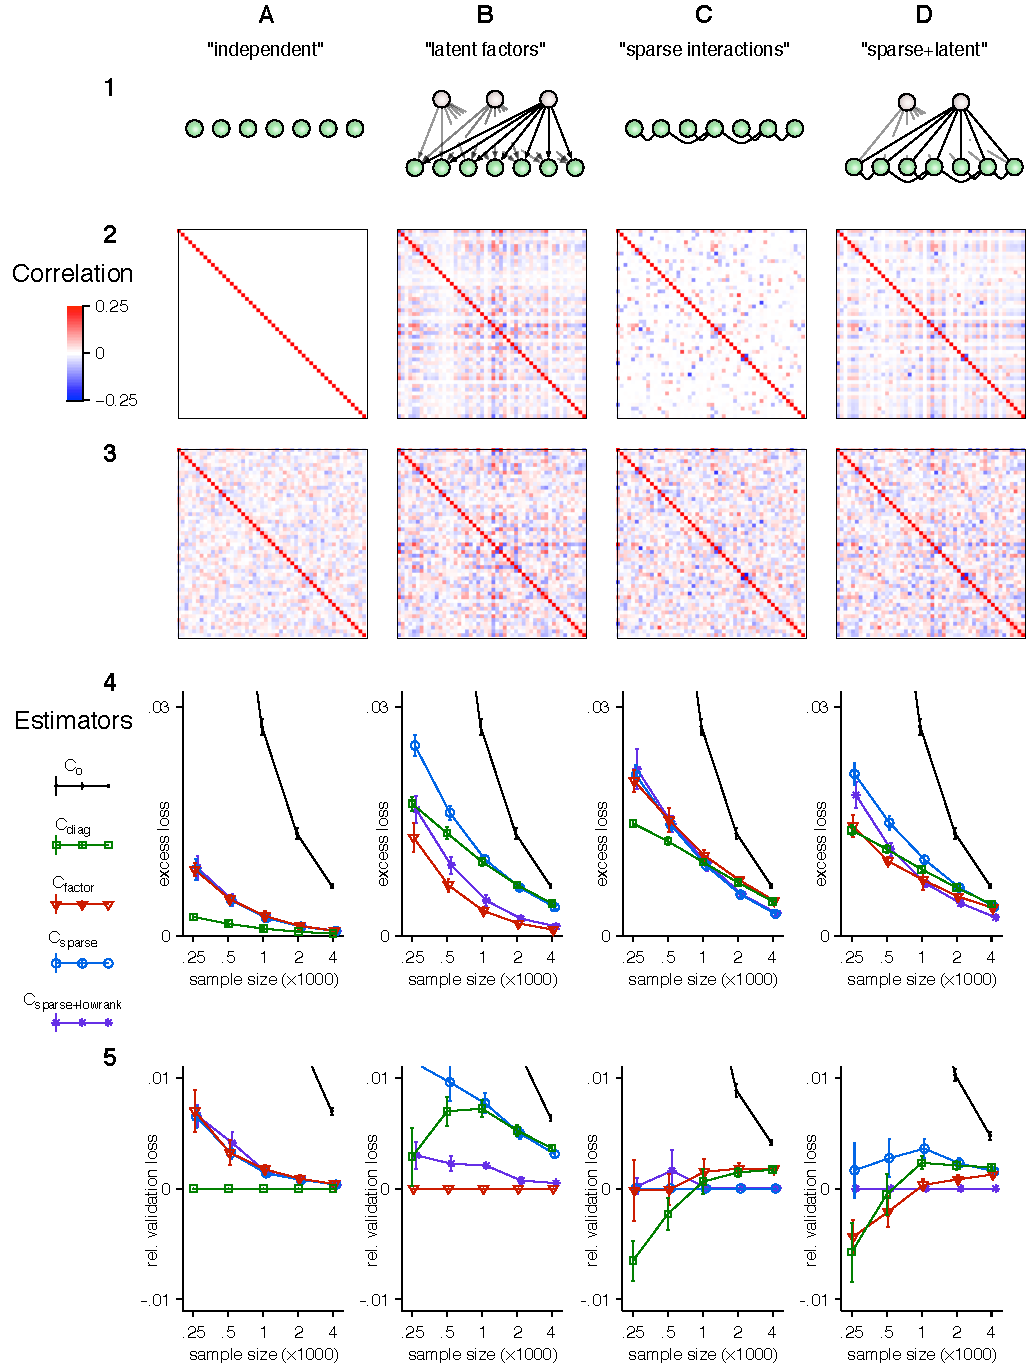
\includegraphics{./figures/Figure02.pdf}
    \end{center}
    \caption{{\bf Regularized estimators whose structure matches the true structure in the data are more efficient.}
    {\bf Row 1.} Graphical representations of the target estimates of the four respective regularized covariance matrix estimators.  Recorded neurons are represented by green spheres and latent units by light-shaded spheres.  Edges represent non-zero partial correlations, \ie \sq{interactions}.
        {\bf Row 1, A}.  For estimator $C_{\sf diag}$, the target estimate is a diagonal matrix, which describes systems that lack linear dependencies. 
        {\bf  Row 1, B.} For estimator $C_{\sf factor}$, the target estimate is a factor model (low-rank matrix plus a diagonal matrix), representing systems in which correlations arise due to common input from latent units. 
        {\bf  Row 1, C}. For estimator $C_{\sf sparse}$, the covariance matrix is approximated as the inverse of a sparse matrix. This approximation describes systems in which correlations arise from a sparse set of  linear associations between the observed units. 
        {\bf  Row 1, D}.  For estimator $C_{\sf sparse+latent}$, the covariance matrix is approximated as the inverse of the sum of a sparse matrix and a low-rank matrix. This approximation describes a model wherein correlations arise due to sparse associations between the recorded cells \emph{and} with several latent units. \\
{\bf Row 2:} Examples of $50\times 50$ correlation matrices corresponding to each structure: {\bf A.} the diagonal correlation matrix, {\bf B.} a factor model with two latent units, {\bf C.}  a correlation matrix with 85\%  off-diagonal zeros in its inverse, and {\bf  D.} a correlation matrix whose inverse is the sum of a rank-1 (\ie one latent unit) matrix and a sparse matrix with 89\% off-diagonal zeros. 
\\
{\bf Row 3:} Sample correlation matrices calculated from samples of size $n=1000$ drawn from simulated random processes with respective correlation matrices shown in Row 2.  The structure of the sample correlation matrix is difficult to discern.
\\
{\bf Row 4:} Correlation matrix estimates computed by estimators with matching structure from the same data as the sample correlation matrices in Row 3. The regularized estimates are closer to the truth than the sample correlation matrices.
\\
{\bf Row 5:} Excess losses (Eq.~\ref{eq:excess-loss}) for the five estimators as a function of sample size. The error bars indicate the standard error of the mean based on 30 samples.  Estimators with structure that matches the true model converged to zero faster than the other estimators. Some exceptions occur when the sample is too small to reveal the structure in the data. In these cases estimators with simpler structures can be more efficient than estimators with true structure.
\\
{\bf Row 6:} Relative cross-validation losses (Eq.~\ref{eq:rel-cv-loss}) for the five estimators with respect to the matching estimator. Error bars indicate the standard error of the mean based on 30 samples.
    }
    \label{fig:1}
\end{FPfigure} 

The target estimate of estimator $C_{\sf diag}$ is the diagonal matrix $D$ containing estimates of neurons' variances. Regularization is achieved by linear \emph{shrinkage} of the unbiased estimate $C_{\sf sample}$ toward $D$ controlled by the scalar \emph{shrinkage intensity} parameter $\lambda \in [0, 1]$:
\begin{equation}\label{eq:c-diag}
C_{\sf diag} = (1-\lambda) C_{\sf sample} + \lambda D
\end{equation}
The structure imposed by $C_{\sf diag}$ favors (performs better  on) populations   with no linear associations between the neurons (\figref{1}{Row 1, A}).  If sample correlations arise from spurious effects, $C_{\sf diag}$ is expected to be more efficient than other estimators. 

The target of estimator $C_{\sf factor}$ is the factor model $L + D$, where $L$ is the $p\times p$ positive \hl{semidefinite} matrix with low rank and $D$ is the diagonal matrix of independent variances.  The estimator, 
\begin{equation}\label{eq:c-factor}
C_{\sf factor} = (1-\lambda) C_{\sf sample} + \lambda (L + D),
\end{equation}
has two hyperparameters: the rank of $L$ (\ie the number of latent factors) and the shrinkage intensity $\lambda$. The structure imposed by $C_{\sf factor}$ favors conditions in which the population activity is linearly driven by a number of latent factors that affect many cells while direct interactions between the recorded cells are insignificant (\figref{1}{Row 1, B}).   

Estimator $C_{\sf sparse}$ is produced by approximating the sample covariance matrix by the inverse of a sparse matrix $S$: 
\begin{equation}\label{eq:c-sparse}
C_{\sf sparse} = S^{-1}.
\end{equation}
Here $S$ is a sparse matrix, \ie one in which a large fraction of off-diagonal elements are set to zero.  The estimator has one hyperparameter that determines the sparsity (fraction of off-diagonal zeros) in $S$. The problem of finding the optimal set of non-zero elements of the precision matrix is known as \emph{covariance selection} \cite{Dempster:1972}. The structure imposed by $C_{\sf sparse}$ favors conditions in which neural correlations arise from direct linear effects (\sq{interactions}) between some pairs of neurons (\figref{1}{Row 1, C}).  


Estimator $C_{\sf sparse+latent}$ is obtained by approximating the sample covariance matrix by a matrix whose inverse is the sum of a sparse component and a low-rank component: 
\begin{equation}\label{eq:c-sl}
C_{\sf sparse+latent} = (S - L)^{-1},
\end{equation}
where, as above, $S$ is a sparse matrix and $L$ is a low rank matrix. The estimator has two hyperparameters: one to regulate the sparsity of $S$ and the other to regulate the rank of $L$. The structure imposed by $C_{\sf sparse+latent}$ favors conditions in which the activity of neurons is determined by linear effects between some observed pairs of neurons and linear effects from several latent units (\figref{1}{Row 1, D}) \cite{Chandrasekaran:2010,Ma:2013}.

We refer to the sparse partial correlations in estimators $C_{\sf sparse}$ and $C_{\sf sparse+latent}$ as \sq{interactions}.

\paragraph{Simulation}
We next demonstrate how the most efficient among different regularized estimators can reveal the structure of correlations.
We constructed four $50\times 50$ covariance matrices, each with structure that matched one of the four regularized estimators (\figref{1}{\,Row 2, A--D}, see Methods for details about how these matrices were generated).  We used these covariance matrices as the ground truth in multivariate normal distributions with zero means and drew samples of various sizes. Even with relatively large sample sizes (\eg $n=1000$), the sample correlation matrices were contaminated by sampling noise and their underlying structures were difficult to discern (\figref{1}{\,Row 3}). 

The evaluation of any covariance matrix estimator, $C$, is performed with respect to a \emph{loss function} $\loss{C,\Sigma}$ to quantify its discrepancy from truth, $\Sigma$.  The loss function must attain its minimum when $C=\Sigma$.

In this study, we adopted the \emph{normal loss} function defined as
\begin{equation}\label{eq:loss}
    \loss{C,\Sigma} = \frac 1 p\left[\ln \det C + \Tr(C^{-1}\Sigma)\right]
\end{equation}

This loss function is related to the multivariate normal log-likelihood function $L(\Sigma|C_{\sf sample})$,
\begin{equation}
     \loss{X,Y} \equiv -\ln(2\pi) - \frac 2 p L(X|Y)
\end{equation}
Normalization by $p$ makes the values of the loss function comparable across different population sizes. 

Although the two functions are similar in form, they differ conceptually: The log-likelihood $L(\Sigma|C_{\sf sample})$ is a function of the parameter $\Sigma$ given the sample covariance matrix $C_{\sf sample}$ whereas the loss function $\loss{C,\Sigma}$ expresses the deviation of an arbitrary estimate $C$ from the truth $\Sigma$.

The choice of the normal loss function is motivated by mathematical convenience. We expect that the main conclusions of our study will not change qualitatively with other well behaved loss functions, such as Stein's entropy loss or quadratic loss \cite{James:1961, Fan:2008, Ledoit:2004, Schafer:2005}.  

The \emph{excess loss} function is produced by shifting the loss function to zero at its minimum:
\begin{equation}\label{eq:excess-loss}
    \eloss{C,\Sigma} = \loss{C,\Sigma}-\loss{\Sigma,\Sigma}
\end{equation}

We drew 30 independent samples of sizes $n=250$, 500, 1000, 2000, and 4000 from each model and computed the excess loss for each of the five estimators.  The hyperparameters of the regularized estimators were optimized by nested cross-validation using only the data in the sample.  All the regularized estimators produced better estimates (lower excess loss) than the sample covariance matrix.  However, estimators whose structure matched the true model typically outperformed the other estimators (\figref{1}{\,row 5}).  There were two exceptions: First, for some smaller samples, the data were insufficient to reveal the true correlation structure and the estimators with simpler structures, $C_{\sf diag}$ and $C_{\sf factor}$, often outperformed the estimators with the matching structure (\figref{1}{\,Row 5, C and D}).  Second, $C_{\sf sparse+latent}$ often performed as well as $C_{\sf sparse}$ on data from models without latent units because it reliably inferred the correct number of latent units: zero.  

With increasing sample sizes, all estimators converged to the truth (zero excess loss).  However, 
the discriminability between their performances increased with sample size (data not shown).

With empirical data, the ground truth, $\Sigma$, is not accessible and excess loss cannot be computed directly. Instead, the loss function must be estimated from the sample through \emph{validation}.  In a validation procedure, an independent \emph{testing sample} is set aside to compute an additional sample covariance estimate $C_{\sf sample}^\prime$ to validate the estimate $C$ computed from the  \emph{training sample}.   The estimate $C_{\sf sample}^\prime$ is used to 
compute the \emph{validation loss} $\loss{C,C_{\sf sample}^\prime}$, which approximates the loss  $\loss{C,\Sigma}$.

The normal loss (Eq.~\ref{eq:loss}) is particularly convenient because it is additive in its second argument, \ie
 \begin{equation*}\label{eq:additivity}
 \loss{C,z_1} + \loss{C,z_2} \equiv \loss{C,z_1+z_2}
 \end{equation*}
With this property of additivity, the validation loss is an unbiased estimate of the loss function:
\begin{equation*}
    \E[C_{\sf sample}^\prime]{\loss{C,C_{\sf sample}^\prime}}=\loss{C,\E[C_{\sf sample}^\prime]{C_{\sf sample}^\prime}}=\loss{C,\Sigma}.
\end{equation*}

The property of additivity does not hold for other popular loss functions such as Stein's entropy loss or various quadratic losses; their validation losses are biased estimates of the loss function. 

Acquiring a separate testing sample is not practical. Instead, $K$-fold cross-validation can be used: The sample is divided into $K$ subsets of approximately equal size ($K=10$ in this study).  Then each subset is used as the validation sample with the other $K-1$ serving as the training sample. The validation losses from all such \sq{folds} are averaged to produce the \emph{cross-validation loss}.  

Cross-validation loss accurately reproduced the relationships between the excess losses of the estimators, with somewhat greater variability (\figref{1}{Row 6}). 

This simulation study demonstrated that, with sufficiently large sample sizes, imposing the correct type of structure on the estimate leads to greater estimation improvement than imposing other structures.

\paragraph{The $C_{\sf sparse+latent}$ estimator is most efficient in neural data}
We recorded the calcium activity of dense populations of neurons in the supragranular layers in primary visual cortex of fentanyl-anesthetized mice using fast random-access 3D scanning two-photon microscopy during visual stimulation (\figref{2}{A--B}) \cite{Reddy:2005, Katona:2012, Cotton:2013}. This technique allowed fast sampling (100--150 Hz) from large numbers (150--350) of cells in a small volume of cortical tissue ($200\times200\times100$ $\mu$m$^3$) in layers 2/3 and 4 (\figref{2}{C}).  The firing rates were inferred using sparse nonnegative deconvolution \cite{Vogelstein:2010} (\figref{2}{C and D}). Only cells that produced detectable calcium activity were included in the analysis (For details, see Methods).  First, 30 repetitions of full-field drifting gratings of 16 directions were presented in random order.  Each grating was presented for 500 ms, without intervening blanks.  This stimulus was used to compute the orientation tuning of the recorded cells (\figref{2}{E}). To estimate the noise correlation matrix, we presented only 2 distinct directions in some experiments or 5 directions in others with between 100 and 300 repetitions of each direction. In this stimulus, each grating lasted 1 second and was followed by a 1-second blank.  The average stimulus response was subtracted from each trial. The traces were then binned into 150 ms intervals for the estimation of the covariance matrix.   The sample correlation coefficients were largely positive and low (average across sites of 0.02 and \hl{less than 0.04 in any site}) (\figref{2}{G} and \figref{5}{D}).  

\begin{figure}    \floatbox[{\capbeside\thisfloatsetup{capbesideposition={right,center},capbesidewidth=8.3cm}}]{figure}[\FBwidth]
    {\caption{{\bf Acquisition of neural signals for the estimation of noise correlations.}
    Visual stimuli comprising full-field drifting gratings interleaved with blank screens ({\bf A}) presented during two-photon recordings of somatic calcium signals using fast 3D random-access microscopy ({\bf B}). 
    {\bf C--G.} Calcium activity data from an example site.
    {\bf C.} Representative calcium signals from eight cells out of 298 cells downsampled to 20 Hz. The inferred firing rate binned in 150 ms intervals are indicated by red ticks below each trace.
    {\bf D.} The raster plot of the inferred firing rates, binned in 150 ms intervals, from the entire population from the first (left) and last (right) minute of the entire recording.  The traces from {\bf C} are highlighted in red.
    {\bf E.} The spatial arrangement and orientation tuning of the 298 cells from the imaged site. Only spiking cells are shown. The cells' colors indicate their orientation preferences. The gray cells were not significantly tuned.
    {\bf F.} The sample noise correlation matrix of the activity of the neural population. 
    {\bf G.} Histogram of noise correlation coefficients. The red line indicates the mean.
} \label{fig:2}}
    {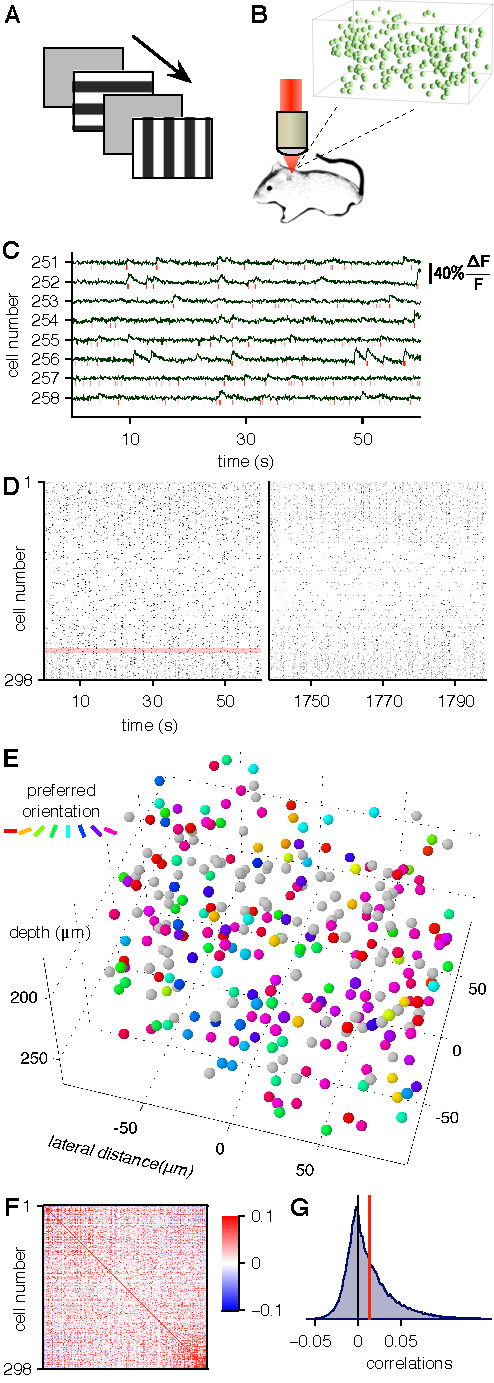
\includegraphics[width=8.3cm]{figures/Figure03.pdf}}
\end{figure}

In these dense populations, direct interactions between cells are likely to influence the patterns of population activity.  We therefore hypothesized that covariance matrix estimators that explicitly modeled the partial correlations between pairs of neurons ($C_{\sf sparse}$ and $C_{\sf sparse+latent}$) would have a performance advantage.  However, the observed neurons must also be strongly influenced by global activity fluctuations and by unobserved common inputs, to the advantage of estimators that explicitly model common fluctuations of the entire population: $C_{\sf factor}$ and $C_{\sf sparse+latent}$.  If both types of effects are significant, then $C_{\sf sparse+latent}$ should outperform the other estimators.

To test this hypothesis, we computed the relative cross-validation loss of estimators  $C_{\sf sample}$, $C_{\sf diag}$, $C_{\sf factor}$, and $C_{\sf sparse}$ with respect to $C_{\sf sparse+latent}$ in $n=27$ imaged sites in 14 mice.  The hyperparameters of each estimator were optimized by nested cross-validation (See Methods for details). Indeed, the sparse+latent estimator outperformed the other estimators (Fig.~\ref{fig:3}). The respective median differences of the cross-validation loss were 0.018, 0.0025, 0.0029, and 0.0017 nats/cell/bin, significantly greater than zero ($p<10^{-5}$ in each comparison, Wilcoxon signed rank test).  

\begin{figure}[!ht]
    \begin{center}
    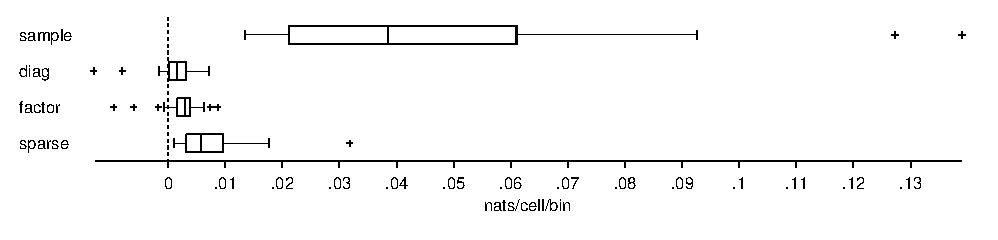
\includegraphics{./figures/src/Fig3.eps}
    \end{center}
    \caption{
    {\bf Cross-validation losses of estimators $C_{\sf sample}$, $C_{\sf diag}$, $C_{\sf factor}$, and $C_{\sf sparse}$ relative to $C_{\sf sparse+latent}$.}
    Covariance estimators $C_{\sf sample}$, $C_{\sf diag}$, $C_{\sf factor}$, and $C_{\sf sparse}$ produced consistently greater validation losses than $C_{\sf sparse+latent}$ ($p<10^{-5}$ in each comparison, Wilcoxon signed rank test, $n=27$ sites in 14 mice). The box plots indicate the $25^{th}$, $50^{th}$, and $75^{th}$ percentiles with the whiskers extending to the minimum and maximum values after excluding the outliers marked with `+'. 
} \label{fig:3}
\end{figure}

Furthermore, $C_{\sf sparse}$ outperformed all the other estimators besides $C_{\sf sparse+latent}$ (Fig.~S\ref{supp:01}) suggesting the greater importance of modeling interactions between pairs of neurons than the common fluctuations of activity across the entire population.

The same evaluation based on the quadratic loss function,
\begin{equation}\label{eq:quadratic}
\loss{C,C_{\sf sample}^\prime}=\frac 1 {p^2}\Tr(C^{-1}C_{\sf sample}^\prime-I)^2,
\end{equation}
instead of the normal loss function reproduced the same relationship between the estimators (Fig.~S\ref{supp:02}). This suggests that the results of this study are robust to the choice of the loss function and do not depend on the assumption of gaussianity. 

\paragraph{Structure of $C_{\sf sparse+latent}$ estimates}
The estimator $C_{\sf sparse+latent}$ separates two sources of correlations: a network of linear interactions between pairs of neurons and a set of latent units reflecting common fluctuations across the entire population.  

We examined the composition of the $C_{\sf sparse+latent}$ estimates at each imaged site (Fig.~\ref{fig:4} and Fig.~\ref{fig:5}). Although the regularized estimates were similar to the sample correlation matrix (\figref{4}{A and D}), the corresponding partial correlation matrices differed substantially (\figref{4}{B and E}). The partial correlation matrix of the regularized estimate was the sum of a sparse component and a low-rank component (\figref{4}{C}).  

In the example site (Fig.~\ref{fig:4}), the sparse component had 89.9\% sparsity (or conversely, 11.1\% connectivity: $connectivity=1-sparsity$) with average node degree of 29.3 (\figref{4}{G}). The average node degree, \ie the average number of interactions linking each neuron, is related to connectivity as $degree = connectivity\cdot(p-1)$, where $p$ is the number of neurons. The low-rank component had rank 71, denoting 71 inferred latent units. The number of latent units and the average node degrees generally increased with population size, although these values varied widely between the datasets (\figref{5}{A and B}). There was an inverse relationship between the number of latent units and the average node degree (\figref{5}{C}): Several sites, despite their large population sizes, were driven by latent units and had few pairwise interactions. This variability may be explained by differences in brain states and recording quality and needs further investigation.

The average partial correlations calculated from these estimates according to Eq.~\ref{eq:partial} at all 31 sites were about 5 times lower than the average sample correlations (\figref{5}{D}). This suggests that correlations between neurons build up from large numbers of small interactions with other neurons. Furthermore, the average partial correlations were less variable: the coefficient of variation of the average sample correlations across sites was 0.41 whereas that of the average partial correlations was 0.35. 

While the sample correlations were mostly positive, the sparse component of the partial correlations (\sq{interactions}) had a high fraction (28.7\% in the example site) of negative values (\figref{4}{F}). This fraction was consistent across multiple sites but the fraction of negative interactions increased with the inferred connectivity \figref{5}{F}.  This increase suggests that negative interactions are inferred only after a sufficient density of positive interactions has been uncovered.

\begin{FPfigure}
    \begin{center}
        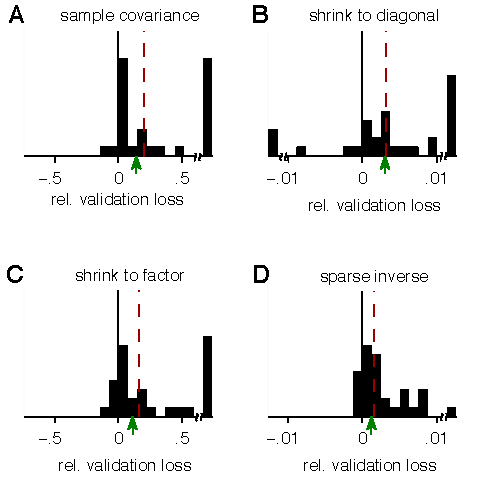
\includegraphics[width=17.35cm]{./figures/Figure04.pdf}
    \end{center}
    \caption{{\bf Example of the structure revealed by $C_{\sf sparse+latent}$ the sparse+latent estimator.}
    {\bf A and B.} The regularized estimate $C_{\sf sparse+latent}$ closely approximates the sample correlation matrix $C_{\sf sample}$. 
    {\bf C and D.} However, the partial correlation matrices from the two estimates differ substantially.
    {\bf E.} The partial correlation matrix of the regularized estimate is decomposed into a sparse component with 89.9\% off-diagonal zeros (bottom-left) and low-rank component of rank 71 (top-right).
    {\bf F.} The sparse component of the regularized partial correlation matrix had little resemblance to the sample correlations: the gray interval indicates the range of correlations containing 89.9\% of cells pairs, equal to the fraction of zeros in the sparse partial correlation matrix. The significant correlations were outside this interval. Yet 51.3\% of the interactions inferred by $C_{\sf sparse+latent}$  linked pairs of neurons whose correlation was below the threshold. Only the remaining 48.7\% of the interactions overlapped with sample correlations above the threshold.
    {\bf G.} A graphical depiction of the positive (green) and negative (magenta) partial correlations as edges between observed neurons. The line density is proportional to the magnitude of the correlation.
    {\bf H.} A subset of neurons from the center of the cluster shown in {\bf G} showing the regularized partial correlations.
    {\bf I.} The same subset with sample correlations thresholded to match the sparsity of the regularized interactions.
}
\label{fig:4}
\end{FPfigure}

Thresholded sample correlations have been used in several studies to infer pairwise interactions \cite{Golshani:2009, Feldt:2011, Malmersjo:2013}.  We therefore compared the interactions inferred by $C_{\sf sparse+latent}$ to those obtained by thresholding the sample correlations with the threshold set to match the connectivity of the $C_{\sf sparse+latent}$ graph.  The networks revealed by the two methods differed substantially. In the example site with 11.1\% connectivity inferred by $C_{\sf sparse+latent}$, only 48.7\% of connections coincided with above-threshold sample correlations (\figref{4}{F, H, and I}). In particular, most of the inferred negative interactions corresponded to low sample correlations (\figref{4}{F}) where high correlations were expected given the rest of the correlation matrix.  This low overlap between the two types of graphs was consistent across the datasets (\figref{5}{E}). 


\begin{figure}    \floatbox[{\capbeside\thisfloatsetup{capbesideposition={right,center},capbesidewidth=8.3cm}}]{figure}[\FBwidth]
    {\caption{{\bf Properties of $C_{\sf sparse+latent}$ estimates from all imaged sites.} 
    Each point represents an imaged site with its color indicating the population size as shown in panels A and B. The example site from Figures \ref{fig:2} and \ref{fig:4} is circled in blue. 
\\
    {\bf A.} The number of inferred latent units vs.~population size.
    {\bf B.} The average node degree for sparse partial correlations vs.~population size.
    {\bf C.} The average node degree in the sparse component in each site vs.~the number of latent units described by the low-rank component of the estimate.
    {\bf D.} The average sample correlations  vs.~the average partial correlations (Eq.~\ref{eq:partial}) of the $C_{\sf sparse+latent}$ estimate.
    {\bf E.} Percent overlap between the graph of highest sample correlations and the graph of interactions inferred by $C_{\sf sparse+latent}$ as a function of the connectivity (\ie $1-sparsity$) of its sparse component. 
    {\bf F.} The percentage of negative interactions vs.~connectivity in the $C_{\sf sparse+latent}$ estimates.
}
\label{fig:5}}
{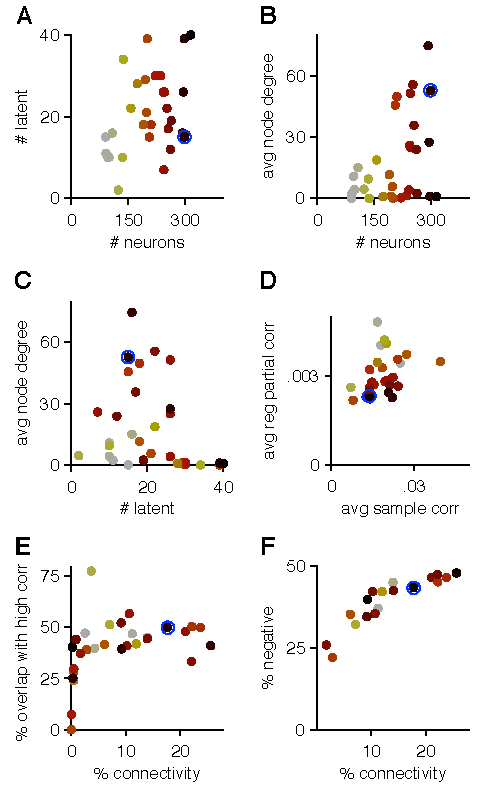
\includegraphics{./figures/Figure06.pdf}}
\end{figure}

\paragraph{Relationship of $C_{\sf sparse+latent}$ to orientation tuning and physical distances}

We also examined the relationship of the correlation structure to the differences in orientation preference and to the physical distances between the cell pairs (Fig.\;\ref{fig:6}).  The partial correlations of the $C_{\sf sparse+latent}$ estimates fell more rapidly with the difference in preferred orientation (\figref{6}{A}) than the sample correlations. They also decreased more rapidly with physical distance, both laterally  (\figref{6}{B}) and in depth (\figref{6}{B}). 

\begin{figure}[!ht]
    \begin{center}
        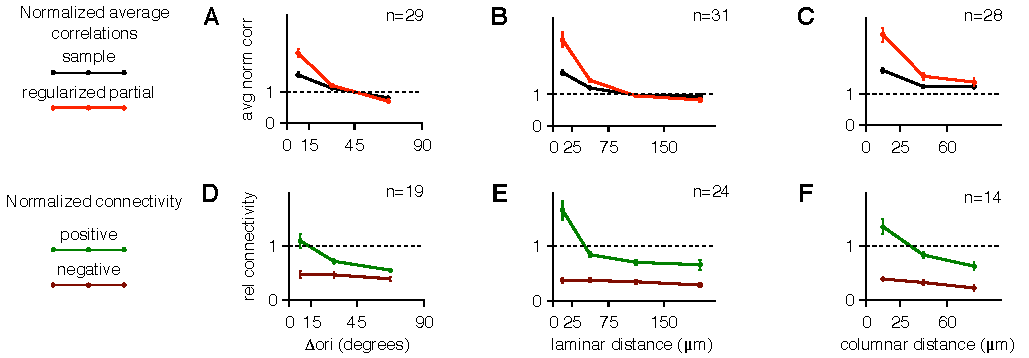
\includegraphics{./figures/Figure07.pdf}
    \end{center}
    \caption{{\bf Dependence of sample correlations and regularized partial correlations on orientation tuning and physical distance.}
    {\bf A--C.} Average partial correlations (red) estimated by $C_{\sf sparse+latent}$ and average sample correlations (black) averaged across multiple imaged sites. At each site the correlations were normalized by the respective average correlation shown in \figref{5}{D}.  The number of sites, $n$, that qualified to be included in the analysis is indicated in each panel. Sites were included if they had at least 20 pairs of neurons in each of the intervals. The error bars indicate the standard error of the mean based on on the number of sites $n$.
    {\bf A.} Average correlations between pairs of neurons tuned to orientation with differences in preferred orientation in the intervals of 0--15$^\circ$, 15--45$^\circ$ and 45--90$^\circ$. 
    {\bf B.} Average correlations between pairs of neurons located at the same depth ($\pm$25$\mu$m) separated by lateral distances in the intervals of 0--25 $\mu$m, 25--75 $\mu$m, 75--150 $\mu$m, and 150+ $\mu$m.
    {\bf C.} Average correlations between pairs of neurons displaced laterally by less than 25 $\mu$m separated in depth by distances in the intervals of 0--25 $\mu$m, 25--60 $\mu$m, and 60+ $\mu$m.
    {\bf D--F.} Normalized connectivity of positive (green) and negative (dark red) interactions from the sparse component obtained from $C_{\sf sparse+latent}$. Normalized connectivity was computed as the fraction of pairs connected by interactions of corresponding signs in each interval divided by the fraction of non-zero interactions across the entire site. }
\label{fig:6}
\end{figure}

The positive and negative interactions in the $C_{\sf sparse+latent}$ estimator were organized differently: The density of the positive interactions fell rapidly with differences in the preferred orientation (\figref{6}{D}), lateral displacements (\figref{6}{E}), and displacement in depth (\figref{6}{F}) whereas the negative interactions were much less selective (\figref{6}{D--F}).

\section*{Discussion}
\paragraph{Functional connectivity as a network of pairwise interactions}
Functional connectivity is often represented as a graph of pairwise interactions. The goal of many studies of functional connectivity was to estimate  anatomical connectivity from  observed multineuronal spiking activity.  For example, characteristic peaks and troughs in the pairwise cross-correlograms of recorded spike trains contain statistical signatures of directional monosynaptic connections and shared synaptic inputs \cite{Gerstein:1964, Perkel:1967, Moore:1970, Alonso:1998, Denman:2013}.  Such signatures are ambiguous as they can arise from network effects other than direct synaptic connections \cite{Aertsen:1989}.  With simultaneous recordings from more neurons, ambiguities can be resolved by inferring the conditional dependencies between pairs of neurons.  Direct causal interactions between neurons produce statistical dependency between them even after conditioning on the state of the remainder of the network and external input. Therefore, conditionally independent neurons can be inferred to lack a direct causal influence.  

Conditional dependencies can be inferred by fitting a probabilistic model of the joint population activity. For example, generalized linear models (GLMs) have been constructed to  include biophysically plausible synaptic integration and membrane kinetics, and individual neurons' stimulus drive~\cite{Pillow:2008}.  Maximum entropy models constrained by observed pairwise correlations also model pairwise coupling between cells \cite{Schneidman:2006, Tkacik:2006, Yu:2008, Tang:2008, Shlens:2009}.  Assuming that the population response follows a multivariate normal distribution, the conditional dependencies between pairs of neurons are expressed by the partial correlations between them.   Each probabilistic model, fitted to the same data may reveal a different network of \sq{interactions},  \ie conditional dependencies between pairs of cells. 

It is not yet clear which approach provides the best correspondence with anatomical connectivity. Little experimental evidence is available to answer this question.  The connectivity graphs inferred by various statistical methods are commonly reported without examining their relation to anatomy.  
Topological properties of such graphs have been interpreted as principles of circuit organization (\emph{e.g.} small-world organization) \cite{Feldt:2011, Yu:2008, Malmersjo:2013}.  However, the topological properties of functional connectivity graphs can depend on the method of inference \cite{Zalesky:2012}. Until a physiological interpretation of functional connectivity is established, the validity of such analyses remains in question and we did not attempt them here.


Inference of the conditional dependencies also depends on the completeness of the recorded population:  To properly condition the pairwise interactions on the activity of the other neurons, we must record from all neurons with which the pair interacts. Unobserved portions of the circuit can introduce false conditional dependencies between observed neurons. For this reason, statistical models of population activity have been most successfully applied to \emph{in vitro} preparations of the retina or cell cultures where high-quality recordings from the complete populations were available \cite{Pillow:2008}. In cortical tissue, electrode arrays record from a small fraction of cells in a given volume, limiting the validity of inference of the pairwise conditional dependencies. This may be the reason that partial correlations have not previously been used to describe the functional connectivity in cortical populations until this study.


Two-photon imaging of population calcium signals presents unique advantages for the estimation of functional connectivity.  While the temporal resolution of calcium signals is limited by calcium dye kinetics, fast imaging techniques combined with spike inference algorithms provide millisecond-scale temporal resolution of single action potentials \cite{Grewe:2010}. However, such high temporal precision comes at the cost of the accuracy of inferred spike rates.  Better accuracy is achieved when calcium signals are analyzed on scales of tens of milliseconds \cite{Cotton:2013}.  The major advantage of calcium imaging is its ability to characterize the spatial arrangement and types of recorded cells.  Recently, advanced imaging techniques have allowed for recordings from nearly every cell in a volume of cortical tissue  \emph{in vivo} \cite{Katona:2012, Cotton:2013} and even from entire nervous systems \cite{Leung:2013, Ahrens:2013}.  These techniques may provide more incisive measurements of functional connectivity than classical electrophysiological recordings.  

The low temporal resolution of calcium signals limits the use of functional connectivity methods that rely on millisecond-scale binning of signals (cross-correlograms, some GLMs, and binary maximum entropy models).  Hence, most studies of functional connectivity have relied on instantaneous sample correlations \cite{Greenberg:2008, Golshani:2009, Hofer:2011, Malmersjo:2013} .  Although some investigators have interpreted such correlations as indicators of (chemical or electrical) synaptic connectivity, most used them as more general indicators of functional connectivity without relating them to underlying mechanisms. 

In our study, we sought to infer pairwise functional connectivity networks  in cortical microcircuits. We hypothesized that partial correlations correspond more closely to underlying mechanisms than sample correlations when recordings are sufficiently dense.  Since neurons form synaptic connections mostly locally and sparsely \cite{Perin:2011}, we \emph{a priori} favored solutions with sparse partial correlations.  The importance of partial correlations may be justified by the principle of maximum entropy: The maximum entropy distribution on discrete or continuous multivariate domains constrained by the observed mean firing rates, their variances, and correlations is the multivariate normal distribution, where the precision matrix specifies the interactions between cell pairs.  Therefore, under the aforementioned assumptions that the recorded population is sufficiently complete and that the model correctly represents the nature of interactions, the network of partial correlations can be hypothesized to be a better representation of functional dependencies than correlations. %\Kcomment{I am not sure about the previous argument.}

\paragraph{Functional connectivity as coactivations}
Another approach to describing the functional connectivity of a circuit is to isolate patterns of multineuronal coactivations \cite{Gerstein:1989, Chapin:1999, Peyrache:2010, Ch:2010, Lopes:2011, Lopes:2013}. Depending on the method of their extraction, coactivation patterns may be referred to as \emph{assemblies}, \emph{factor loadings}, \emph{principal components}, \emph{independent components}, \emph{activity modes}, \emph{eigenvectors}, or \emph{coactivation maps}. Coactivation patterns could be interpreted as signatures of Hebbian cell assemblies \cite{Gerstein:1989, Ch:2010}, \ie groups of tightly interconnected groups of cells involved in a common computation.  Coactivation patterns could also result from shared input from unobserved parts of the circuit, or global network fluctuations modulating the activity of the local circuit \cite{Okun:2012}.

Coactivation patterns and pairwise connectivity are not mutually exclusive since assemblies arise from patterns of synaptic connectivity.  However, an analysis of coactivation shifts the focus from detailed interactions to  collective behavior.  
In our study, the functional connectivity through modes of coactivations was represented by the factor analysis estimator $C_{\sf factor}$.  

\paragraph{Combining pairwise interactions and coactivations}
In the effort to account for the joint activity patterns that are poorly explained by pairwise interactions, investigators have augmented models of pairwise interactions with additional mechanisms such as latent variables \cite{Koster:2013},  high-order correlations \cite{Ganmor:2011}, or global network fluctuations \cite{Tkacik:2013}.

In our study, we combined pairwise interactions with collective coactivations by applying the recently developed numerical techniques for the inference of the partial correlation structure in systems with latent variables \cite{Chandrasekaran:2010, Ma:2013}.  The resulting estimator, $C_{\sf sparse+latent}$, effectively decomposed the functional connectivity into a sparse network of pairwise interactions and coactivation mode vectors.

\paragraph{Addressing ill-posedness}
Inferring the conditional dependencies between variables in a probabilistic model is an ill-posed problem: small variations in the data produce large errors in the inferred network of dependencies. The problem becomes worse as the number of  recorded neurons increases until such models lose their statistical validity \cite{Roudi:2009}.  As techniques have improved to allow recording from larger neuronal populations, experimental neuroscientists have addressed this problem by extending the recording durations to keep sampling noise in check and verified that existing models are not overfitted and that the stationarity assumption is observed\cite{Tkacik:2013}. However, ambitious projects, such as the BRAIN initiative  \cite{Alivisatos:2013}, aim to record from significantly larger populations. Simply increasing recording duration will not be sufficient, and the problem must be addressed by using regularized estimators. Regularization biases the solution toward a small subspace to counteract the effect of  sampling noise in the empirical data. However, biasing the solution to an inappropriate subspace does not allow significant estimation improvement and hinders interpretation.

Several strategies have been developed to limit the model space in order to improve the quality of the estimate. For example, Ganmor et al. \cite{Ganmor:2011} developed a heuristic rule to identify the most significant features that must be fitted by a maximum entropy model for improved performance in retina. Generalized linear models typically employ $L_1$ penalty terms to constrain the solution space and to effectively reduce the dimensionality of the solution \cite{Pillow:2008}.  

In our study, regularization was also accomplished by dimensionality reduction (feature selection) schemes to produce sparse, constrained solutions.


\paragraph{Model selection}
We evaluated the covariance matrix estimators using the cross-validated normal log likelihood.  However, this does not limit the applicability of its conclusions to normal distributions. Indeed our major findings could be reproduced using other loss functions (compare Fig.~\ref{fig:3} and Fig.~S\ref{supp:02}).  Other probabilistic models, fitted to the same data, would also serve as estimators of the covariance matrix.  If a different model yields better estimation of the covariance matrix than the estimator proposed here, we believe that its structure should deserve consideration as the better representation of the functional connectivity.

The results of model selection must be interpreted with caution.  As we demonstrated by simulation, with limited data, an incorrect but more constrained model can produce a better estimate than a more complex model with correct representation of dependencies.   Therefore, showing that a more constrained model has better cross-validated performance than a more complex model does not necessarily support the conclusion that it reveals a better representation of dependencies in the data.  This caveat is related to \emph{Stein's Paradox} \cite{Efron:1977}: The biasing of an estimate toward an arbitrary low-dimensional target is guaranteed to produce \emph{some} improvement over the best estimate with many degrees of freedom.

\paragraph{Physiological interpretation and future directions}

Here we showed that among several models a sparse network of linear interactions with several latent inputs yielded the best estimates of the noise covariance matrix for cortical microcircuits.  This finding is valuable in itself: improved estimates of the noise covariance matrix for large datasets are important in order to understand the role of noise correlations in population coding \cite{Abbott:1999, Sompolinsky:2001, Averbeck:2006, Ecker:2011}  

Moreover, this estimation approach provides a graphical representation of the dependencies in the data that can be used to formulate and test hypotheses about the structure of connectivity in the microcircuit. Importantly, the inferred functional interactions were substantially different from the network of the most significant sample correlations \figref{4}{F, H, and I}.  For example, the $C_{\sf sparse+latent}$ estimator reveals a large number of negative interactions that were not present in the sample correlation matrix (\figref{4}{F}) and may reflect inhibitory circuitry.  Although the network of functional interactions inferred by the optimal estimator, $C_{\sf sparse+latent}$, will not be identical to the anatomical connectivity, it may accurately reflect average connectivity profiles. Future experiments utilizing molecular markers for different cell types and follow-up multiple whole-cell \emph{in vitro} experiments \cite{Hofer:2011, Ko:2013} will directly compare the inferred functional connectivity graphs to the underlying anatomical circuitry. Finally, the latent units inferred by the estimator can be analyzed for their physiological interpretation. For example, these latent units may be modulated under different brain states (e.g. slow-wave sleep, attention) and stimulus conditions (e.g. certain types of stimuli may engage feedback connections). 

\section*{Methods}
% You may title this section "Methods" or "Models". 
% "Models" is not a valid title for PLoS ONE authors. However, PLoS ONE
% authors may use "Analysis" 
\paragraph{Ethics statement}
All procedures were conducted in accordance with the ethical guidelines of the National Institutes of Health and were approved by the Baylor College of Medicine IACUC. 

\paragraph{Surgery and two-photon imaging}
The surgical procedures and data acquisition were performed as descrbed in \cite{Cotton:2013}. Briefly, C57BL/6J mice (aged p40--60) were used. Anesthesia was initiated with isoflurane (3\%) and maintained with the mixture of fentanyl (0.05 mg/kg), midazolam (5 mg/kg), and medetomidine (0.5 mg/kg), with boosts of half the initial dose every 3 hours.  A craniotomy was performed over the right primary visual cortex.  Membrane-permeant calcium indicator Oregon Green 488 BAPTA-1 AM (OGB-1, Invitrogen) was loaded by bolus injection.  The craniotomy was sealed using a glass coverslip secured with dental cement. 

Calcium imaging began 1 hour after dye injection.  All imaging was performed using the 3D-RAMP two-photon microscope as described in \cite{Cotton:2013}. First, a 3D stack was acquired and cells were manually segmented. Then calcium signal were collected by sampling in the center of each cell at rates of 100 Hz or higher, depending on the number of cells.

\paragraph{Visual stimulus}
The visual stimulus consisted of full-field drifting gratings with 90\% contrast, luminance of 10 cd/m$^2$, spatial frequency of 0.08 cycles/degree, and temporal frequency of 2 cycles/s. Two sets of stimuli were presented for each imaging site: the first to map directional tuning and the second to estimate noise correlations. Directional tuning was mapped using a pseudo-random sequence of drifting gratings at sixteen equally spaced directions of motion, 500 ms per direction, for 3 min without blanks. The data for covariance estimation were collected during presentations of full-field drifting gratings with the same parameters as those used in directional tuning except only two directions (in 9 datasets) or five directions (in 22 datasets) were used and the presentations lasted 1 second and were separated by 1-second blanks.  Each stimulus condition was presented between 100 and 300 times.
\paragraph{Data processing}
All data were processed in MATLAB using the DataJoint data processing chain toolbox ({\tt datajoint.github.com}) first developed in our lab. 

The collected fluorescent traces were deconvolved to reconstruct the firing rates for each neuron. First, the first principal component was subtracted from the traces, which reduced common mode noise related to small cardiovascular movements \cite{Cotton:2013}. The resulting traces were low-pass filtered below 0.1 Hz and downsampled to 20 Hz. Firing rates were estimated using a fast non-negative deconvolution algorithm \cite{Vogelstein:2010}.

Orientation tuning was computed by fitting the mean firing rates in response to gratings drifting in directions $\phi$ with two-peaked von Mises tuning functions of the form $f(\phi)=a + b\exp\left[\frac 1 w(\cos(\phi-\theta)-1) \right] + c\exp\left[\frac 1 w(\cos(\phi-\theta+\pi)-1) \right]$ where $b\ge c$ are the amplitudes of the two respective peaks, $w$ is the tuning width, and  $\theta$ is the preferred direction. The significance of the fit was determined by the permutation test: the labels of the direction were randomly permuted 10,000 times.  The $p$-value of the fit was computed as the fraction of the permuted datasets for which the $R^2$ value of the tuning function fit exceeded that of the real data.  Cells were considered tuned with $p$-values below 0.05.

For covariance estimation, the analysis was limited to the period with 2 or 5 stimulus conditions and lasted between 14 and 27 minutes (mean 22 minutes).  Cells that did not have substantial spiking activity (those whose variance was less than 2\% of the $90^{th}$ percentile in each site) were excluded from the analysis.

\paragraph{Cross-validation}
To compare the performance of the estimators against each other, we used conventional 10-fold cross validation. Briefly, each recording was split into 30 blocks of equal duration.  The 30 blocks were then grouped randomly into 10 datasets with 3 blocks in each.  This splitting of the data was chosen to achieve a high degree of independence between the 10 datasets for cross-validaton purposes. Splitting the data into smaller blocks could increase dependencies between them due to temporal correlations thereby violating the assumptions of cross-validation. Then, each dataset was used as the testing dataset with the rest of the data used for estimating the covariance matrix.  

Since each of the regularized estimators had one or two hyperparameters, we used \emph{nested cross-validation}:  The outer loop evaluated the performance of the estimators with the optimal hyperparameter values estimated within the inner loop.  Hyperparameters were optimized by a two-phase search algorithm: random search to find a good starting point followed by pattern search to find the global minimum.  The inner cross-validation loop subdivided the training dataset from the outer loop to perform 10-fold cross-validation in order to evaluate each choice of the hyperparameter values.  Thus the size of the training dataset within the inner loop comprised 81\% of the entire recording.

When the cross-validation loss was not required, only the inner loop of cross-validation was used, applied to the entire dataset.  This approach was used to compute the covariance matrix estimates and their excess-loss in the simulation study (\figref{1}{\,Rows 4 and 5}) and to analyze the partial correlation structure of the sparse+latent estimator (Fig.~\ref{fig:4}--\ref{fig:6}).
\paragraph{Covariance estimation}
Within the inner loop of cross-validation, covariance matrix estimation was performed with fixed hyperparameter values provided by the search algorithm.  The computation of regularized estimators only required the sample covariance matrix $C_{\sf sample}$ of the training dataset. 

Estimator $C_{\sf diag}$ (Eq.~\ref{eq:c-diag})  used two hyperparameters: the covariance shrinkage intensity $\lambda \in [0,1]$ and variance shrinkage intensity $\alpha \in [0,1]$.  The variances (the diagonal of $C_{\sf sample}$) were shrunk toward (linearly mixed with) their mean value:
\begin{equation}
D = (1-\alpha)C_{\sf sample}\circ I + \alpha \frac 1 p \Tr(C_{\sf sample}) I
\end{equation}
Then the diagonal matrix $D$ was used as the target of covariance shrinkage (Eq.~\ref{eq:c-diag}) to produce the final regularized estimate.  The {\tt corpcor} package in the programming language R also implements this estimator \cite{Schafer:2010}, although its analytical optimization of the shrinkage intensities is based on the mean squared error whereas we optimized them with respect to the normal loss function (Eq.~\ref{eq:loss}).

Estimator $C_{\sf factor}$ used two hyperparameters: the number of latent factors $d$ and the shrinkage intensity $\lambda \in [0, 1]$.  
The matrix $L$ of rank $d$ and the diagonal matrix of individual variances $D$ were computed by solving the minimization problem
\begin{equation}
(L,D) = \argmin\limits_{\tilde L,\tilde D} \loss{\tilde L + \tilde D,C_{\sf sample}},
\end{equation}
which we solved by an expectation-maximization (EM) algorithm.  Under our chosen loss function (Eq.~\ref{eq:loss}), this is equivalent to maximum likelihood estimation of $L$ and $D$ under the multivariate Gaussian distribution.  The final regularized estimate is obtained by linear shrinkage toward the factor model (Eq.~\ref{eq:c-factor}). 

Estimator $C_{\sf sparse}$  has one hyperparameter $\lambda$ to regulate the sparsity of its precision matrix $S$. The precision matrix is computed in two steps: First, the zero structure is determined by minimizing the $L_1$-penalized loss:
\begin{equation}
Z = \argmin\limits_{\tilde Z \succ 0} \loss{{\tilde Z}^{-1},C_{\sf sample}} + \lambda \|\tilde Z \|_1
\end{equation}
where $\tilde Z\succ 0$ denotes the constraint that $\tilde Z$ be a positive definite matrix and $\|\tilde Z\|_1$ is the element-wise $L_1$ norm of the matrix $\tilde Z$. This problem formulation is known as \emph{graphical lasso} \cite{Meinshausen:2006, Friedman:2008}. To solve this minimization problem, we modified the alternative-direction method of multipliers (ADMM) algorithm \cite{Ma:2013}. 
Then, after the zero structure was determined, the remaining coefficients were fitted without penalty:
\begin{equation}
S = \argmin\limits_{\tilde S \in Z^\sharp} \loss{\tilde S,C_{\sf sample}},
\end{equation}
where $Z^\sharp$ denotes the set of positive-definite matrices with the same zero structure as $Z$.  This step was also solved by ADMM.  Then the final estimate is the inverse of $S$ (Eq.~\ref{eq:c-sparse}). Unlike $C_{\sf diag}$ and $C_{\sf factor}$, this estimator does not include linear shrinkage: the selection of the sparsity level provides sufficient flexibility to fine tune the regularization level.

Estimator $C_{\sf sparse+latent}$ has two hyperparameters: the number of latent units $d$ and \hl{hyperparameter $\lambda$ regulating the sparsity level}. $C_{\sf sparse+latent}$ estimates a larger sparse precision matrix $S^\ast$ of the joint distribution of the $p$ observed neurons and $d$ latent units.  
\begin{equation}
S^\ast=
\begin{pmatrix}
S & S_{12} \\
S_{12}^\T & S_{22}
\end{pmatrix},
\end{equation}
where the $p\times p$ partition $S$ corresponds to the visible units and expresses their partial correlation structure, and $S_{12}$ and $S_{22}$ are of size $p\times d$ and $d\times d$, respectively. 
Then the covariance matrix of the observed population is 
\begin{equation}
C_{\sf sparse+latent} = \left(S-S_{12}S_{22}^{-1}S_{12}^\T\right)^{-1}
\end{equation}
The $p\times p$  matrix $L=S_{12}S_{22}^{-1}S_{12}^\T$ has rank $d$. Rather than searching for the optimal sparse structure of $S_{12}$ and $S_{22}$, an ill-posed problem, we estimated these components together as the low-rank matrix $L$.

The estimate is found in two steps. First, we use the ADMM algorithm to find the zero structure of $S$ by minimizing the $L_1$-penalized loss \cite{Chandrasekaran:2010,Ma:2013}:
\begin{equation}
(Z,\cdot) = \argmin\limits_{\tilde Z,\tilde L} \loss{\tilde Z-\tilde L, C_{\sf sample}} + \lambda\|\tilde Z\|_1
\end{equation}
Then we find the sparse and low-rank components of the precision matrix by solving (also using ADMM) 
\begin{equation}
(S,L) = \argmin\limits_{\tilde S \in Z^\sharp,\tilde L} \loss{\tilde S-\tilde L, C_{\sf sample} }
\end{equation}

The partial correlation matrix with both sparse and low-rank components is computed from $C_{\sf sparse+latent}$ according to Eq.~\ref{eq:partial}; it includes the effects of interactions between the visible and latent units.  This estimate of the partial correlations was used in analyses of average partial correlations (\figref{4}{B and E} and \figref{5}{D}, and \figref{6}{A--C}).  The sparse component $S$ was used separately in analyses of the connectivity graphs (\figref{4}{F, G, H} and \figref{5}{B, C, E, and F} and \figref{6}{D--F}); in this case, the partial correlations were computed by normalizing the sparse component alone without the low-rank component: 
\begin{equation}
P_{\sf sparse} = -(S\circ I)^{-\frac 1 2} S  (S\circ I)^{-\frac 1 2}
\end{equation}

The MATLAB code for these computations is available at {\tt http://github.com/atlab/cov-est}.


\paragraph{Simulation}
For simulation, ground truth covariance matrices were produced by taking 150 independent samples from an artificial population of 50 independent, identically normally distributed units. The covariance matrices were then subjected to the respective regularizations to produce the ground truth matrices for the simulation studies (\figref{1}{\,Row 2}). Samples were then drawn from multivariate normal distributions with the respective true covariance matrices to be estimated by each of the estimators. 

\section*{Acknowledgments}
We thank Genevera Allen for a helpful discussion, and Eftychios Pnevmatikakis for helpful suggestions and feedback on the manuscript.  This work was supported by grants NEI R01-EY018847, NEI P30-EY002520-33, NEI T32-EY07001-37, NIDA R01DA028525, the NIH-Pioneer award DP1-OD008301 to AST, the McKnight Scholar Award to AST; the Arnold \& Beckman Foundation Young Investigator Award to AST; and NSF grants DMS-0817649, DMS-1122094 to KJ.
% The bibtex filename
\bibliography{references.bib}


%\section*{Figure Legends}
\newpage
\section*{Supporting Information}
\setcounter{figure}{0}
\renewcommand{\figurename}{Figure S}


\begin{FPfigure}
\begin{center}
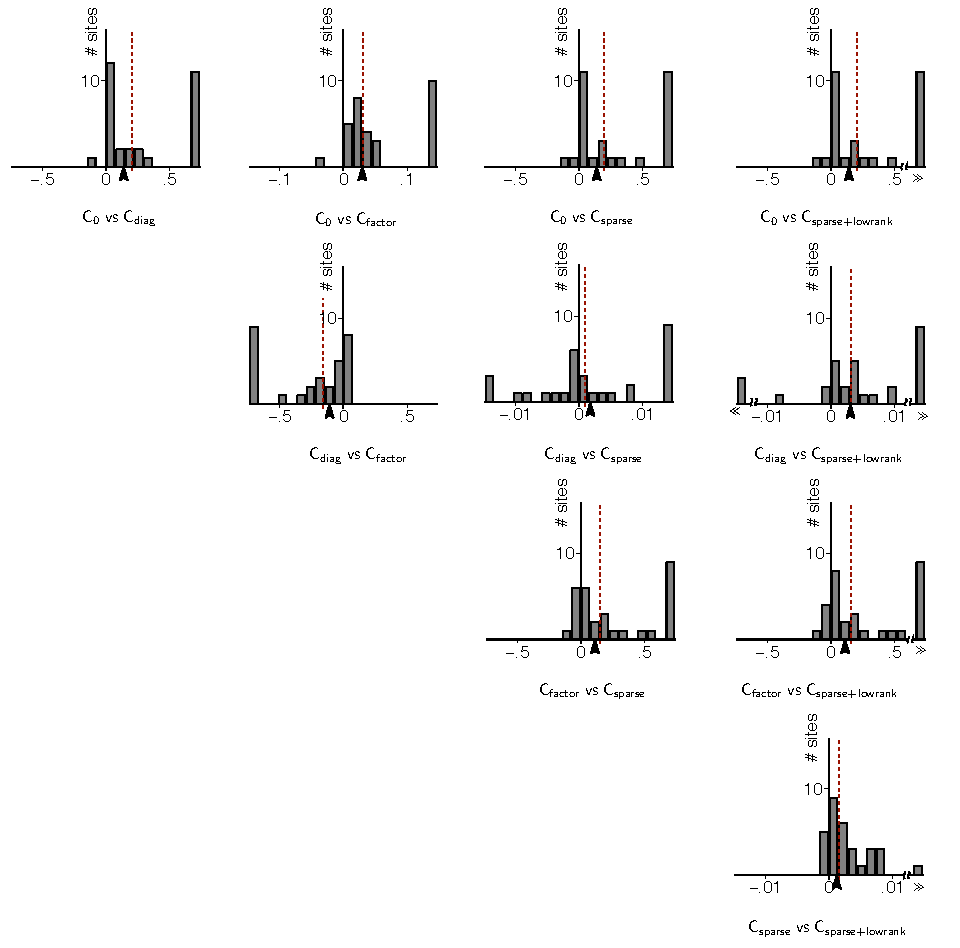
\includegraphics{./figures/Figure-Supp01.pdf}
\end{center}
\caption{{\bf All-to-all performance comparisons of the sample covariance matrix and the four regularized estimators with respect to multivariate normal cross-validation loss.}
\\{\bf A--D.} These panels are identical to those in \figref{3}{A--D}.
\\{\bf E.} $C_{\sf sparse}$ outperforms $C_{\sf sample}$: median improvement 0.15 nats/neuron, $p=3.9\times 10^{-5}$.
\\{\bf F.} $C_{\sf sparse}$ performs similarly to $C_{\sf diag}$: median improvement $1.0\times10^{-3}$ nats/neuron, $p=0.13$.
\\{\bf G.} $C_{\sf sparse}$ outperforms $C_{\sf factor}$: median improvement $0.15$ nats/neuron, $p=1.2\times10^{-4}$.
\\{\bf H.} $C_{\sf factor}$ outperforms $C_{\sf sample}$: median improvement $0.029$ nats/neuron, $p=2.7\times10^{-4}$.
\\{\bf I.} $C_{\sf factor}$ performs worse than $C_{\sf diag}$: median improvement $-0.16$ nats/neuron, $p=1.6\times10^{-4}$.
\\{\bf J.} $C_{\sf diag}$ outperforms $C_{\sf sample}$: median improvement $0.14$ nats/neuron, $p=2.7\times10^{-5}$.
}
\label{supp:01}
\end{FPfigure}


\begin{figure}[!ht]
\floatbox[{\capbeside\thisfloatsetup{capbesideposition={right,center},capbesidewidth=8.3cm}}]{figure}[\FBwidth]
{\caption{{\bf The sparse+latent estimator outperforms the other estimators under the quadratic loss (Eq.~\ref{eq:quadratic}) just as it did under the normal loss (Eq.~\ref{eq:loss}) used in Fig.~\ref{fig:3}.}
    Histograms of the cross-validation loss of estimators $C_{\sf sample}$, $C_{\sf diag}$, $C_{\sf factor}$, and $C_{\sf sparse}$ with respect to $C_{\sf sparse+latent}$ using the quadratic loss function.
    The histograms were obtained from 31 imaged sites in 15 mice. 
    All medians (red dashed lines) were significantly greater than zero, indicating the dominance of $C_{\sf sparse+latent}$ over the other estimators. 
    The arrow heads indicate the results for the site shown in Fig.~\ref{fig:2} and Fig.~\ref{fig:4}.
    The $p$-values are for the two-sided Wilcoxon's signed rank test.
    \\{\bf A.} $C_{\sf sparse+latent}$ outperforms $C_{\sf sample}$: median $\Delta\ell_{C_{\sf sample},C_{\sf sparse+latent}}$ = 0.35, $p=1.7\times 10^{-6}$.
    \\{\bf B.} $C_{\sf sparse+latent}$ outperforms $C_{\sf diag}$: median $\Delta\ell_{C_{\sf diag},C_{\sf sparse+latent}}$ = $2.5\times 10^{-3}$, $p=1.0\times 10^{-4}$.
    \\{\bf C.} $C_{\sf sparse+latent}$ outperforms $C_{\sf factor}$: median $\Delta\ell_{C_{\sf factor},C_{\sf sparse+latent}}$ = 0.27, $p=1.2\times 10^{-6}$.
    \\{\bf D.} $C_{\sf sparse+latent}$ outperforms $C_{\sf sparse}$: median $\Delta\ell_{C_{\sf sparse},C_{\sf sparse+latent}}$ = $3.7\times 10^{-4}$, $p=2.2\times 10^{-3}$.
}
\label{supp:02}}
{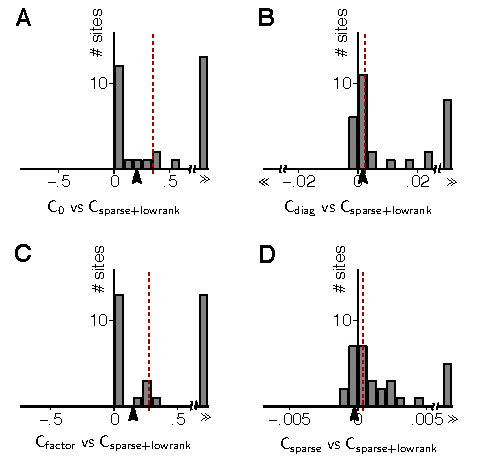
\includegraphics{./figures/Figure-Supp02.pdf}}
\end{figure}


\end{document}

